\documentclass[11pt]{article}

%%% PACKAGES %%%

%% ## Page Layout ## %%
\usepackage[a4paper,left=2.8cm,right=2.8cm,top=2.3cm,bottom=2.3cm]{geometry}
\usepackage{marginnote}

%% ## Sprog og tengsætning ## %%
\usepackage[utf8]{inputenc}					%  Input encoding af tegnsæt, gør det muligt at bruge æøå
\usepackage[english]{babel}					% Dokumentets sprog
\usepackage[T1]{fontenc} 					% Output encoding af tegnsæt
\usepackage{textcomp}						% Obsolete ????
\usepackage[normalem]{ulem}					% strikethrough with \sout{...}

%% ## Font ## %%
%%Default, but with more...
\usepackage{lmodern}
%% Baskerville, use together with \usepackage[T1]{fontenc}
%\usepackage{baskervillef}
%\usepackage[varqu,varl,var0]{inconsolata}
%\usepackage[scale=.95,type1]{cabin}
%\usepackage[baskerville,vvarbb]{newtxmath}
%\usepackage[cal=boondoxo]{mathalfa}
%% Mera Mono
%\usepackage[scaled]{beramono}
%% Courier
\usepackage{courier}
\usepackage{weva}								% Some handwriting font

%% ## gib Tables ## %%
\usepackage{array}
\usepackage{tabu}

\usepackage{enumitem}

\usepackage{blindtext}							% Dummy text with \blintext, 
\usepackage{layout}

%% ## something ## %%
\usepackage{setspace}							% Controls spacing between lines, and gives access to enviroments
%\singlespacing
\onehalfspacing
%\doublespacing

%% ## Gib Colors ## %% 
\usepackage[dvipsnames,table]{xcolor}			% Define color with this command \definecolor{name}{model}{color-spec} ### With table(colortbl) loaded, we can now change color in tables
\definecolor{myOrange}{RGB}{253,136,36}
\definecolor{rammuDark}{RGB}{44,62,80}
\definecolor{rammuRed}{RGB}{231,76,60}
\definecolor{rammuBlueD}{RGB}{41,128,185}
\definecolor{rammuBlueL}{RGB}{52,152,219}
\definecolor{pink}{RGB}{255,80,255}
\definecolor{myDarkGrey}{gray}{0.2}
\definecolor{myGrey}{gray}{0.3}
\definecolor{myPink}{RGB}{181,0,184}
\definecolor{myLightBlue}{RGB}{31,144,201}
\definecolor{anotherOrange}{RGB}{255,140,0}

\usepackage{soul}								% Hightlight text with \hl
\DeclareRobustCommand{\hlgreen}[1]{{\sethlcolor{green}\hl{#1}}}
\DeclareRobustCommand{\hlmagenta}[1]{{\sethlcolor{pink}\hl{#1}}}

%% ## Links ## %%
\usepackage[colorlinks]{hyperref}
\hypersetup{
	colorlinks = true,
	linkcolor = black,
	citecolor = black,
	urlcolor = black,
	}

%% ## Insert Pictures/Graphics
\usepackage{graphicx}

%% ## Custom shit
\usepackage{sectsty}							% Makes is possible to change section color
\sectionfont{\color{anotherOrange}}
\subsectionfont{\color{myLightBlue}}
\subsubsectionfont{\color{myPink}}

%\hbadness = 10000 								% Går så vi slipper se på underfull \hbox, burde ikke ændre på måden dokumentet bliver lavet på...

% Changes to way unnumbered footnotes look
\makeatletter
\renewcommand*{\@fnsymbol}[1]{\ensuremath{\ifcase#1\or \dagger\or \dagger\or \ddagger\or
    \mathsection\or \mathparagraph\or \|\or **\or \dagger\dagger
    \or \ddagger\ddagger \else\@ctrerr\fi}}
\makeatother



\begin{document}

\pagenumbering{Roman}
\title{Cisco IOS Commands for CCNA}
\date{\today}
\author{Ajers}

\maketitle

\phantomsection
\tableofcontents
\pagebreak

\pagenumbering{arabic}

\section{IOS Modes and Navigation}

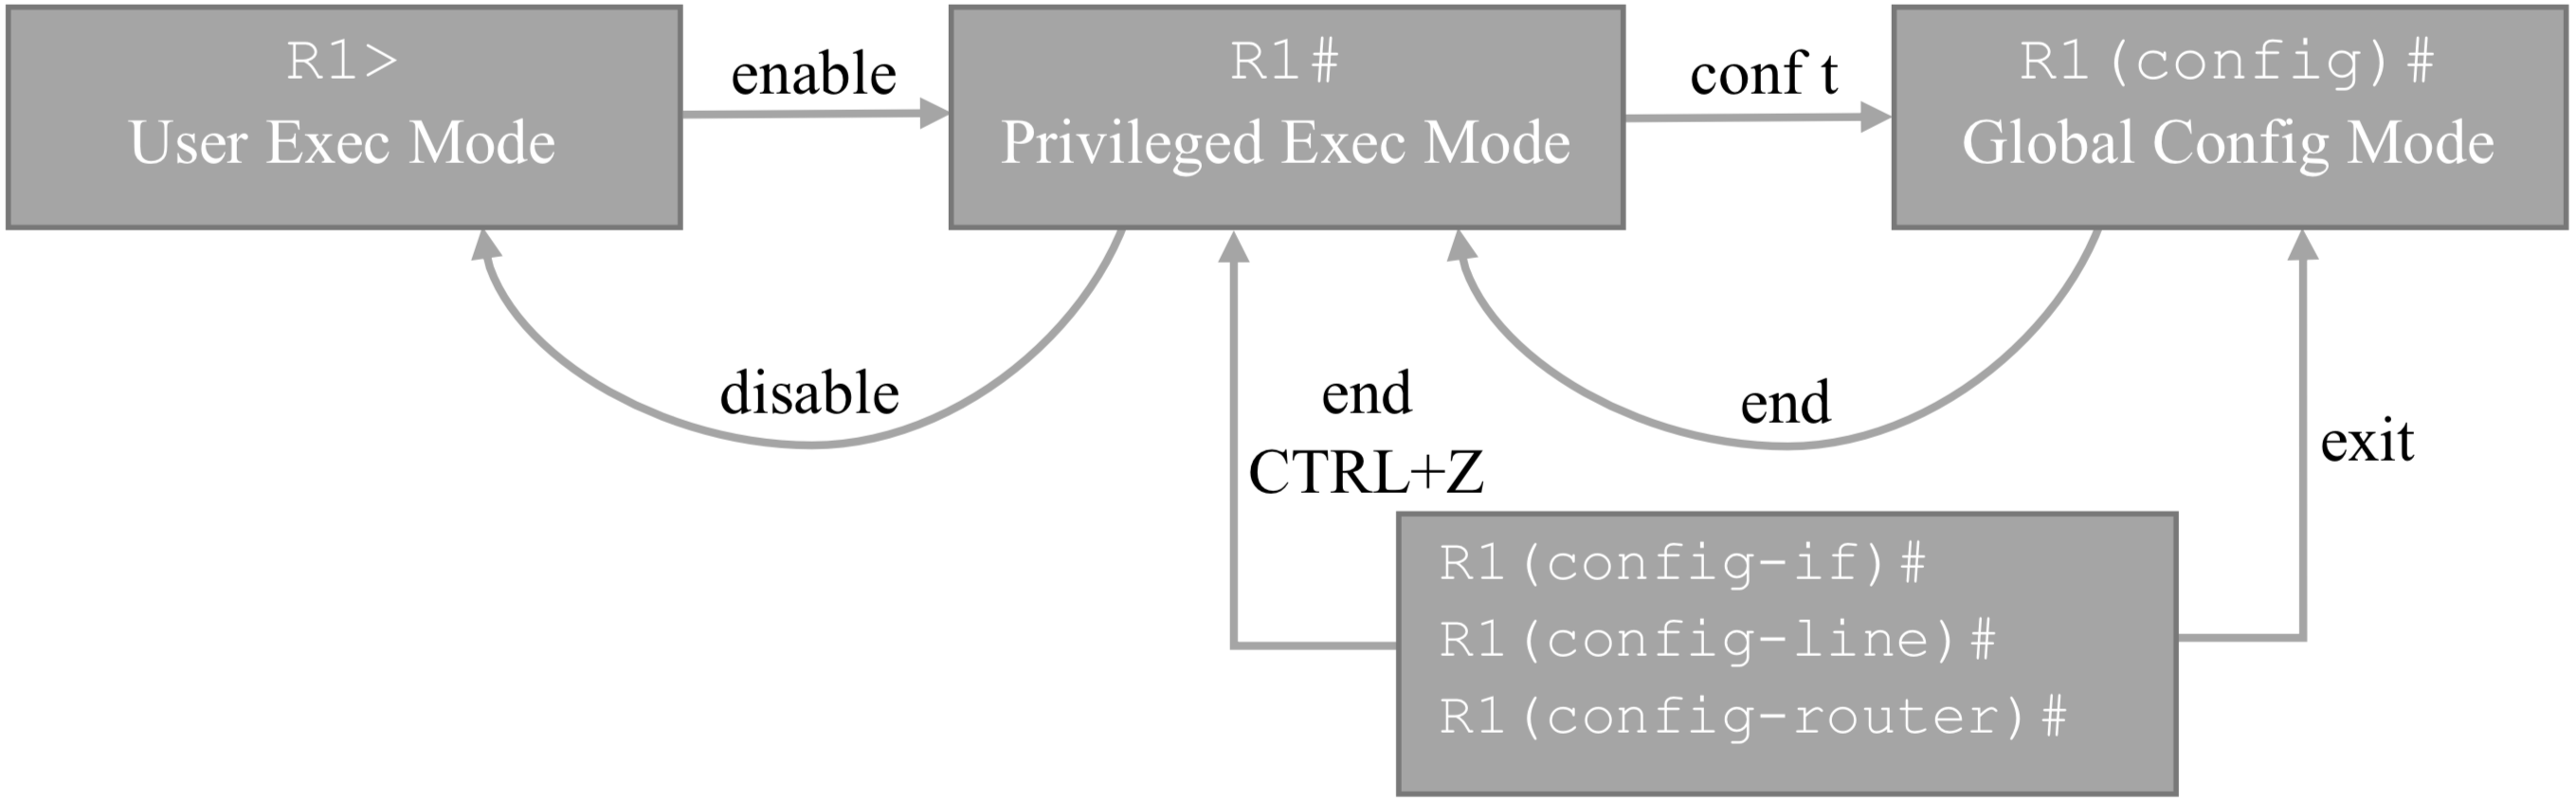
\includegraphics[width=\textwidth]{pics/mode-and-nav}

\noindent
When describing the use of commands, I generally use the conventions shown in \autoref{tab:ioscommandstructure}

\begin{table}[h]
{\tabulinesep=1mm			%Does something with space between rows
\parindent0pt				%No indentation for the table
\begin{tabu}{ | l | X | }
	\hline
	\texttt{Normal/\textbf{Bold}} & Normal/\textbf{Bold} text indicates commands and keywords that you enter literally as shown.\\ \hline
	\texttt{\textit{Italics}} & Italic text indicates arguments for which you supply values. \\ \hline
	\texttt{[x]} & Square brackets indicate an optional element (keyword or argument). \\ \hline
	\texttt{\{x\}} & Braces indiacte a required element (keyword or argument). \\ \hline
	\texttt{[x\{y|z\}]} & Braces and vertical lines within square brackets indicate a required choice within an optional element. \\
	\hline

\end{tabu}}
	\caption{}
	\label{tab:ioscommandstructure}
\end{table}

\section{Basic Setup}
\subsection{Hostname}
\ttfamily
	(config)\# hostname \textit{hostname} \\
	(config)\# hostname no hostname\footnote{Removes the hostname.}
	
\subsection{User Exec Password}
	(config)\# line console 0\textrm{\footnote{0 indicates the first, and properly only console port.}} \\
	(config-line)\# password \textit{password} \\
	(config-line)\# login\footnote{Enables user EXEC access} \\
	(config-line)\# exit
	
\subsection{Privileged Exec Password}
	(config)\# enable secret \textit{secret\_password}\\
	(config)\# exit
	
\subsection{VTY Line Password}
	(config)\# line vty 0 15 \\
	(config-line)\# password \textit{password} \\
	(config-line)\# login\footnote{Enables VTY access}

\subsection{Encrypt Passwords}
(config)\# service password-encryption

\subsection{SVI (Switch Virtual Interface) Configuration}
(config)\# interface vlan \textit{vlan\_id} \\
(config-if)\# ip address \textit{ip\_address} \textit{subnetmask} \\
(config-if)\# no shutdown

\subsection{Default Gateway on a Switch}
(config)\# ip default-gateway \textit{gateway\_address}

\subsection{Description on an interface}
(config-if)\# description \textit{desired\_description}

\subsection{Enable Router to forward IPv6 packets}
(config)\# ipv6 unicast-routing

\subsection{IPv6 link-local}
(config-if)\# ipv6 address \textit{ipv6\_address} link-local

\subsection{Banner Message}
(config)\# banner motd \# hello, this is the message. Choose a \\character that will start and end the message text, in this \\case the hashtag \#

\subsection{Save running config}
\# Copy running-config startup-config

\section{Miscellaneous}
\subsection{Stop dem Lookups (Disable DNS Lookup)}
(config)\# no ip domain-lookup

\subsection{If you fucked up}
\# erase startup-config \\
\# delete vlan.dat\footnote{If present, check with ``dir flash:''}\\
\# reload

\subsection{Disable CPD (Cisco Descovery Protocol)}
(config)\# no cdp run

\subsection{Logging Synchronous}
(config)\# line console 0 \\
(config-line)\# logging synchronous

\subsection{Set Console Time to Never Timeout}
(config)\# line console 0 \\
(config-line)\# exec-timeout 0 0\footnote{first 0 is for minutes, second is for seconds}

\section{Backing up and restoring TFTP (Trivial File Transfer Protocol)}
\# copy running-config/startup-config tftp\\
Enter IP address of the target server:\\
Enter desired name for the file:\\
Press ‘Enter’ to confirm\vspace{11pt}\\
\# copy tftp running-config/startup-config \\
Enter the IP address of the host where the configuration file is \\stored:\\
Enter the name to assign to the configuration file: \\
Press ‘Enter’ to confirm

\section{Configuring SSH}
\textrm{The device needs an unique hostname}\\
(config)\# ip domain-name \textit{name.something}\\
(config)\# crypto key generate rsa\footnote{Enter desired key length (1024)}\\
(config)\# ip ssh version 2\\
(config)\# username \textit{name} secret \textit{secret\_password}\vspace{11pt}\\
(config)\# ip ssh time-out 60\\
(config)\# ip ssh authentication-retries 2\vspace{11pt}\\
(config)\# line vty 0 15\\
(config-line)\# login local\footnote{Remote login now looks for local user for authentication}\\
(config-line)\# transport input ssh\footnote{Only able to remote via SSH}

\subsection{Delete RSA key pair and disables SSH server}
(config)\# crypto key zerosize rsa
\section{VLAN}
\subsection{Configure more than 1 interface}
(config)\# interface range \textit{type} \textit{first-number} - \textit{last-number}

\subsection{Create VLAN}
(config)\# vlan \textit{vlan\_id}\\
(config-vlan)\# name \textit{vlan\_name}\\
(config-vlan)\# end/exit

\subsection{Assign Ports to VLANs}
(config)\# interface \textit{interface\_id}\\
(config-if)\# switchport mode access\\
(config-if)\# switchport access vlan \textit{vlan\_id}\\
(config-if)\# end/exit
\subsubsection*{Change Port to VLAN 1}
(config-if)\# no switchport access vlan

\subsection{Delete VLAN}
(config)\# no vlan \textit{vlan\_id}

\subsection{Trunk Configuration}
(config)\# inteface \textit{interface\_id}\\
\sout{(config-if)\# switchport trunk encapsulation dot1q}\footnote{Old Command}\\
(config-if)\# switchport mode trunk
\subsubsection*{Specify a Native VLAN Other Than VLAN 1}
(config-if)\# switchport trunk native vlan \textit{vlan\_id}
\subsubsection*{Specify VLANs Allowed On The Trunk Link}
(config-if)\# switchport trunk allowed vlan \textit{vlan\_list}

\subsection{Restting Configured Values on the Trunk Links}
\subsubsection*{Set Trunk To Allow All VLANs}
(config)\# inteface \textit{interface\_id}\\
(config-if)\# no switchport trunk allowed vlan
\subsubsection*{Reset Native VLAN to Default}
(config)\# inteface \textit{interface\_id}\\
(config-if)\# no switchport trunk native vlan

\subsection{To enable trunking from a Cisco switch to a device that does not support DTP (Dynamic Trunking Protocol)}
(config-if)\# switchport mode trunk\\
(config-if)\# switchport nonegotiate

\subsection{Private VLAN (PVLAN)}
\subsubsection*{Enable Protected Port}
(config-if)\# switchport protected
\subsubsection*{Disable Protected Port}
(config-if)\# no switchport protected

\section{Inter VLAN Routing}
\subsection{Router-on-a-Stick}
\doublespacing
\textrm{\sout{Start by enabling Trunking on the switchport connected to the router. Disable DTP.}\\Create a subinterface for a VLAN}\\
(config)\# interface \textit{interface\_id.subinterface\_id}\\
\textrm{Assign subinterface to a VLAN}\\
(config-subif)\# encapsulation dot1q \textit{vlan\_id} [native]\\
\textrm{Assign IP address range}\\
(config-subif)\# ip address \textit{ip\_addres subnet\_mask}\\
\textrm{When all the subinterfaces have been configured, turn on the physical port}\\
(config)\# interface \textit{interface\_id}\\
(config-if)\# no shutdown

\section{Switching Security}
\subsection{DHCP Snooping}
\textrm{Enable globally}\\
(config)\# ip dhcp snooping\\
\textrm{Enable on specific VLAN}\\
(config)\# ip dhcp vlan \textit{number1}, \textit{number2}\\
\textrm{Trust a specific interface}\\
(config)\# interface \textit{type} \textit{interfaceidnumber}\\
(config-if)\# ip dhcp trust\\
\textrm{(Optional) Limit the rate at which an attacker can continually send bogus DHCP requests through untrusted ports to the DHCP server}\\
(config-if)\# ip dhcp snooping limit rate \textit{rate}

\subsection{Port Security}
\textrm{First we have to convert the port(s) to an access port(s), otherwise we can’t do port security on it}\\
(config-if)\# switchport mode access\\
\textrm{Limit the number of mac-addresses on the port – default is 1}\\
(config-if)\# switchport port-security maximum \textit{number}\\
\textrm{Set violation type (look at \autoref*{tab:violationtypes}) - default is shutdown}\\
(config-if)\# switchport port-security violation \{ protect | \\restrict | shutdown \}\\
\textrm{Turn on sticky mac addresses (dynamically learned and added to the running config)}\\
(config-if)\# switchport port-security mac-address sticky [\textit{mac-adr}]\\
\textrm{Lastly turn on port security}\\
(config-if)\# switchport port-security

\begin{table}[h]
\tabulinesep=1mm			%Does something with space between rows
\parindent0pt				%No indentation for the table
%\ttfamily
\begin{tabu}{| X | X | X | X | X | X |}
	\hline
	Violation Mode & Forwards Traffic & Sends Syslog Message & Displays Error Messages & Increases Violation Counter & Shuts Down Port\\ \hline
	Protect & No & No & No & No & No \\ \hline
	Restrict & No & Yes & No & Yes & No \\ \hline
	Shutdown & No & No & No & Yes & Yes \\
	\hline
\end{tabu}
\caption{Violation Types}
\label{tab:violationtypes}
\end{table}

\onehalfspacing
\section{Show and Verify -- VLAN}
\subsection{Trunk Configuration}
\# show interfaces \textit{interface\_id} switchport\\
\# show interfaces trunk

\subsection{DTP Mode}
\# show dtp interface \textit{interface\_id}

\subsection{Troubleshooting Trunks}
\# show interfaces \textit{interface\_id} trunk

\subsection{Missing VLANs}
\subsubsection*{Is port in correct VLAN}
\# show vlan\\
\# show mac address-table
\subsubsection*{VLAN present in VLAN database}
\# show vlan\\
\# show interfaces\\
\# show interfaces switchport

\subsection{Port Security Settings}
\# show port-security interface \textit{interface\_id}

\subsection{Secure MAC Addresses}
\# show port-security address

\subsection{Routing Table}
\# show ip route\\
\# show ip route static\\
\# show ip route \textit{network}\vspace{11pt}\\  
\# show ipv6 route\\
\# show ipv6 route static\\
\# show ipv6 route \textit{network}


\section{Static Routing}
(config)\# ip route \textit{network\_address} \textit{subnet\_mask} \{\textit{ip\_address} | \\\textit{interface\_type} \textit{interface\_number} [\textit{ip\_address}]\} [\textit{distance}] \\{[name \textit{name}]} [permamnent] [tag \textit{tag}]

\subsection{IPv4}
\subsubsection*{Next-Hop Static Route (Recursive Static Route????)}
(config)\# ip route \textit{target\_network subnet\_mask next\_hop\_ip\_addr}
\subsubsection*{Directly Attached/Connected Static Route}
(config)\# ip route \textit{target\_network subnet\_mask exit\_int}
\subsubsection*{Fully Specified Static Route}
(config)\# ip route \textit{target\_network subnet\_mask exit\_int next\_\\hop\_ip\_addr}
\subsubsection*{Default Static Route}
(config)\# ip route 0.0.0.0 0.0.0.0 \{\textit{exit\_int} | \textit{next\_hop\_ip}\}\\
\textrm{\textbf{NOTE:} An IPv4 default static route is commonly referred to as a quad-zero.}

\subsection{IPv6}
\textrm{\textbf{NOTE:} IPv6 routing must be enabled with} (config)\# ipv6 unicas- routing\vspace{11pt}\\
(config)\# ipv6 route \textit{ipv6-prefix/prefix-lenght} \{\textit{ipv6-addr} | \\\textit{exit-int}\}
\subsubsection*{Next-Hop Static Route}
(config)\# ipv6 route \textit{ipv6-prefix/prefix-lenght} \textit{next-hop-ipv6-addr}
\subsubsection*{Directly Attached/Connected Static Route}
(config)\# ipv6 route \textit{ipv6-prefix/prefix-lenght} \textit{exit-int}
\subsubsection*{Fully Specified Static Route}
(config)\# ipv6 route \textit{ipv6-prefix/prefix-lenght} \textit{ipv6-addr} \textit{exit-int}
\subsubsection*{Default Static Route}
(config)\# ipv6 route ::/0 \{\textit{ipv6-addr} | \textit{exit-int}\}

\subsection{Summary Route IPv4}
\textrm{First we need to calculate the summary route, which can be done in 3 steps:\\
\textbf{Step 1:} List the networks in binary format.\\
\textbf{Step 2:} Count the number of far-left matching bits to determine the mask for the summary route. This is the prefix, or subnet mask for the summarized route i.e.\ /14 or 255.252.0.0\\
\textbf{Step 3:} Copy the matching bits and add zero-bits to determine the summarized network address.
}
\subsubsection*{Example}
\textrm{\textbf{Step 1:}}\\
172.20.0.0\qquad 10101100.00010100.00000000.00000000\\
172.21.0.0\qquad 10101100.00010101.00000000.00000000\\
172.22.0.0\qquad 10101100.00010110.00000000.00000000\\
172.23.0.0\qquad 10101100.00010111.00000000.00000000\\
\textrm{\textbf{Step 2:}}\\
172.20.0.0\qquad \textcolor{cyan}{10101100.000101}00.00000000.00000000\\
172.21.0.0\qquad \textcolor{cyan}{10101100.000101}01.00000000.00000000\\
172.22.0.0\qquad \textcolor{cyan}{10101100.000101}10.00000000.00000000\\
172.23.0.0\qquad \textcolor{cyan}{10101100.000101}11.00000000.00000000\\
\textrm{14 matching bits = /14 or 255.252.0.0\\\textbf{Step 3:}}\\
10101100.000101 \textrm{= matching bits\\Add zero-bits:}\\
10101100.000101\textcolor{pink}{00.00000000.00000000}\\
\textrm{\textbf{Answer} = 172.20.0.0\\Enter the summary route as you would a normal static route, with the summary route as the target network:}\\
(config)\# ip route 172.20.0.0 255.252.0.0 \{\textit{exit-int} | \textit{next-hop}\}

\subsection{Summary Route IPv6}
\textrm{Summarizing IPv6 networks into a single IPv6 prefix and prefix-length can be done in seven steps:\\
\textbf{Step 1.} List the network addresses (prefixes) and identify the part where the addresses differ.\\
\textbf{Step 2.} Expand the IPv6 if it is abbreviated.\\
\textbf{Step 3.} Convert the differing section from hex to binary.\\
\textbf{Step 4.} Count the number of far left matching bits to determine the prefix-length for the summary route. The summary can also be determined by converting just the lowest and highest network addresses to binary to find the matching bits.\\
\textbf{Step 5.} Copy the matching bits and then add zero bits to determine the summarized network address (prefix).\\
\textbf{Step 6.} Convert the binary section back to hex.\\
\textbf{Step 7.} Append the prefix of the summary route (result of Step 4).
}

\subsection{Floating Static Route}
\textrm{This is a default static route that is configured with the \texttt{[distance]} sat higher than 1 (default), with another default static route with a distance of 1. Because the value is greater than 1, the route floats and is not present in the routing table, inless the preferred route fails.}
\section{RIP - Routing Information Protocol}
\section{Single Area OSPF}
\subsection{IPv4}
\subsubsection*{Enter and enable OSPF with}
(config)\# \textbf{router ospf} \textit{process\_id}\vspace{4pt}\\
\textrm{The \texttt{\textit{process-id}} value represents a number between 1 and 65,535 and is selected by the network administrator. The \texttt{\textit{process-id}} value is locally significant, which means that it does not have to be the same value on the other OSPF routers to establish adjacencies with those neighbors.}
\subsubsection*{Give the router an ID}
(config-router)\# \textbf{router-id} \textit{rid}\vspace{4pt}\\
\textrm{The rid value is any 32-bit value expressed as an IPv4 address, e.g.} (config-router)\# router-id 1.1.1.1
\subsubsection*{If the router already has a name, you might have to clear the OSPF process before you can change it}
(config-router)\# router-id 1.1.1.1\vspace{11pt}\\
\%\%\% Some error message\vspace{11pt}\\
\# clear ip ospf process\\
\textrm{Press \texttt{y} to the prompt}\vspace{11pt}\\
show ip protocols | section Router ID -> to see the change

\subsubsection*{Using a Loopback Interface as the Router ID}
(config)\# interface loopback 0\\
(config-if)\# ip address 1.1.1.1 255.255.255.255\\
(config-if)\# end\\
\textrm{The IPv4 address of the loopback interface should be configured using a 32-bit subnet mask (255.255.255.255). This effectively creates a host route. A 32-bit host route does not get advertised as a route to other OSPF routers. 
The example displays how to configure a loopback interface with a host route on R1. R1 uses the host route as its router ID, assuming there is no router ID explicitly configured or previously learned.
}
\subsubsection*{Enabling OSPF on interfaces}
\textrm{The \texttt{network} command determines which interfaces participate in the routing process for an OSPF area. Any interfaces on the router that match the network address in the \texttt{network} command are enabled to send and receive OSPF packets. As a result, the network (or subnet) addresses for the interface is included in OSPF routing updates. The basic command syntax is}\vspace{8pt}\\
(config-router)\#\textbf{network} \textit{network\_address wildcard\_mask} \textbf{area} \textit{area\_id}\vspace{11pt}\\
\textrm{The \texttt{\textbf{area} \textit{area\_id}} syntax refers to the OSPF area. When configuring single-area OSPF, the \texttt{\textbf{network}} command must be configured with the same \texttt{area\_id} value on all routers. Although any area ID can be used, it is good practice to use an area ID of 0 with single-area OSPF. This convention makes it easier if the network is later altered to support multiarea OSPF.}\vspace{8pt}\\
(config)\# router ospf 10\\
(config-router)\# network 172.16.1.0 0.0.0.255 area 0\\
(config-router)\# network 172.16.3.0 0.0.0.3 area 0\\
(config-router)\# network 192.168.10.4 0.0.0.3 area 0\vspace{11pt}\\
\textrm{As an alternative, OSPFv2 can be enabled using the \texttt{\textbf{network} \textit{int\_ip\_address} \\\textbf{0.0.0.0} \textbf{area} \textit{area\_id}} router configuration mode command.\\
Below you can see an example of specifying the interface IPv4 address with a quad 0 wildcard mask. Entering \texttt{network 172.16.3.1 0.0.0.0 area 0} on R1 tells the router to enable interface Serial0/0/0 for the routing process. As a result, the OSPFv2 process will advertise the network that is on this interface (172.16.3.0/30).\\
The advantage of specifying the interface is that the wildcard mask calculation is not necessary. OSPFv2 uses the interface address and subnet mask to determine the network to advertise.\\
\textbf{Note:} This method is not really used by Cisco.}\vspace{8pt}\\
(config)\# router ospf 10\\
(config-router)\# network 172.16.1.1 0.0.0.0 area 0\\
(config-router)\# network 172.16.3.1 0.0.0.0 area 0\\
(config-router)\# network 192.168.10.5 0.0.0.0 area 0
\subsubsection*{Propagate the default route}
(config-router)\# \textbf{default-information originate}
\subsubsection*{Passive Interface}
(config-router)\#\textbf{ passive-interface} \textit{interface\_id}
\subsubsection*{Adjusting the interface bandwidth}
(config)\# \textbf{interface} \textit{interface\_id}\\
(config-if)\# \textbf{bandwidth} \textit{kilobits}
\subsubsection*{Manually setting the OSPF cost}
(config)\# \textbf{interface} \textit{interface\_id}\\
(config-if)\# \textbf{ip ospf cost} \textit{value}
\subsubsection*{Some show commands}
show ip ospf neighbor\\
show ip protocols\\
show ip ospf\\
show ip ospf interface\\
show ip ospf interface brief\\
show ip ospf interface serial 0/0/1

\subsection{IPv6}

\section{EIGRP}
\subsection{Protocol Configuration}
(config)\# \textbf{router eigrp} \textit{asn}\footnote{The \textit{asn} (autonomous system number) argument can be assigned to any 16-bit value between the number 1 and 65,535. All routers within the EIGRP routing domain must use the same autonomous system number.}\vspace{11pt}\\
\textrm{Set the Router ID}\\
(config-router)\# \textbf{eigrp router-id} \textit{ipv4\_address}\footnote{The IPv4 address used to indicate the router ID is actually any 32-bit number displayed in dotted-decimal notation, excluding 0.0.0.0 and 255.255.255.255.}\vspace{11pt}\\
\textrm{Add networks to advertise}\\
(config-router)\# \textbf{network} \textit{network\_address} [\textit{wildcard\_mask}]\vspace{11pt}\\
\textrm{Designate passive interfaces}\\
(config-router)\# \textbf{passive-interface} \{\textit{interface\_id} | \textbf{default\footnote{The \textit{default} keyword sets all interfaces as passive.}}\}\vspace{11pt}\\
\textrm{Propagate a default static route}\\
(config-router)\# \textbf{redistribute static}\vspace{11pt}\\
\textrm{Disable automatic route summarization}\\
(config-router)\# \textbf{no auto-summary}\vspace{11pt}\\
\textrm{Configure K values to manipulate metric formula}\\
(config-router)\# \textbf{metric weights 0} \textit{k1 k2 k3 k4 k5}
\subsection{Interface Configuration}
(config)\# \textbf{interface} \textit{interface\_id}\vspace{11pt}\\
\textrm{Configure the bandwidth parameter}\\
(config-if)\# \textbf{bandwidth} \textit{kilobits\_bandwidth\_value}\footnote{Default value is 1544 kb/s.}\vspace{11pt}\\
\textrm{Configure EIGRP Manual Summarization}\footnote{Configure the summary route on all interfaces that send EIGRP packets.}\\
(config-if)\# \textbf{ip summary-address eigrp} \textit{asn network\_address \\subnet\_mask}\vspace{11pt}\\
\textrm{Set maximum bandwidth EIGRP can consume}\\
(config-if)\# \textbf{ip bandwidth-percent eigrp} \textit{asn percentage}\vspace{11pt}\\
\textrm{Configure hello and hold timers}\\
(config)\# \textbf{ip hello-interval eigrp} \textit{asn seconds}\\
(config)\# \textbf{ip hold-time eigrp} \textit{asn seconds}
\subsection{MD5 Authentication}
(config)\# \textbf{key chain} \textit{name\_of\_chain}\\
(config-keychain)\# \textbf{key} \textit{key\_id}\footnote{ The key ID is the number used to identify an authentication key within a keychain. The range of keys is from 0 to 2,147,483,647. It is recommended that the key number be the same on all routers in the configuration.}\\
(config-keychain-key)\# \textbf{key-string} \textit{key\_string\_text}\footnote{The key string is similar to a password. Routers exchanging authentication keys must be configured using the same key string.}
\subsubsection*{Enable MD5 on an interface}
(config)\# \textbf{interface} \textit{interface\_id}\\
(config-if)\# \textbf{ip authentication mode eigrp} \textit{asn} \textbf{md5}\\
(config-if)\# \textbf{ip authentication key-chain eigrp} \textit{asn name\_of\_chain}
\subsection{Troubleshooting}
show ip eigrp interfaces\\
show ip eigrp neighbors\\
show ip eigrp topology\\
show ip eigrp traffic\\
clear ip eigrp neighbors
\section{Point-to-Point Connections}
\subsection{HDLC - High-Level Data Link Control}
\textrm{Cisco uses HDLC as the default encapsulation method on synchronous serial lines. But if it has been changed, change it back with:}\vspace{4pt}\\
(config-if)\# \textbf{encapsulation hdlc}

\subsection{PPP - Point-to-Point Protocol}
\subsubsection*{Enable PPP on an interface}
(config-if)\# \textbf{encapsulation ppp}
\subsubsection*{PAP}
\textrm{For PAP to work, you need a user on the router}\vspace{4pt}\\
(config)\# \textbf{username} \textit{user\_XX} \textbf{secret} \textit{passw\_XX}\\
(config)\# \textbf{interface} \textit{interface\_id}\\
(config-if)\#\textbf{ ppp authentication pap}\\
(config-if)\# \textbf{ppp pap sent-username} \textit{user\_YY} \textbf{password} \textit{passw\_YY}\vspace{11pt}\\
\textrm{Mirror these settings at the other end of the link}\vspace{4pt}\\
(config)\# \textbf{username} \textit{user\_YY} \textbf{secret} \textit{passw\_YY}\\
(config)\# \textbf{interface} \textit{interface\_id}\\
(config-if)\# \textbf{ppp authentication pap}\\
(config-if)\# \textbf{ppp pap sent-username} \textit{user\_XX} \textbf{password} \textit{passw\_XX}
\subsubsection*{CHAP}
\textrm{The hostname on one router must match the username the other router has configured. The password on the 2 users must also match.}\vspace{4pt}\\
(config)\# \textbf{username} \textit{username} \textbf{password} \textit{password}\\
(config)\# \textbf{interface} \textit{interface\_id}\\
(config-if)\# \textbf{ppp authentication chap}
\subsection{Troubleshoot}
\subsubsection*{Clock rate}
\textrm{The DCE end has to provide the clock signal, look for it under interface serial in the running config.}\\
\# show running-config | begin interface Serial\vspace{11pt}\\
\textrm{If it has not been set, set it like this:}\vspace{1pt}\\
(config-if)\# \textbf{clock rate} \textit{clock\_rate}
\subsubsection*{Authentication}
\textrm{Use the same command as above, look for encapsulation and authentication.\\ Use the debug command to find further errors.}\\
\# debug ppp authentication\vspace{11pt}\\
\textrm{Disbale all debugging with}\\
\# undebug all
\subsubsection*{Some other shit}
\textrm{Find users}\\
\# show run | include user\vspace{11pt}\\
show interfaces\\
show interfaces serial\\
show ppp multilink
\section{GRE - Generic Routing Encapsulation}
(config)\# \textbf{interface tunnel} \textit{tunnel\_id\_number}\\
(config-if)\# \textbf{tunnel source} \textit{ip\_address}\\
(config-if)\# \textbf{tunnel destination} \textit{ip\_address}\\
(config-if)\# \textbf{ip address} \textit{ip\_address mask}\footnote{Specifies the IP address of the tunnel interface.}\\
{[}(config-if)\# \textbf{tunnel mode gre ip}]
\subsection{Troubleshooting}
show ip interface brief | include Tunnel\\
show interface tunnel \textit{tunnel\_id\_number}\\
show ip ospf neighbor
\section{NTP}
\textrm{[Optional] Change timezone to CET}\\
(config)\# \textbf{clock timezone CET +1}\vspace{11pt}\\
\textrm{Set the time manually}\\
\# \textbf{clock set} \textit{hh:mm:ss day\_of\_month 3\_letter\_month year}\vspace{11pt}\\
\textrm{Configure the IOS device to be a NTP server}\\
(config)\# \textbf{ntp master} \textit{number}\vspace{11pt}\\
\textrm{Get time from a NTP server}\\
(config)\# \textbf{ntp server} \textit{ip\_address}
\section{Syslog}
\textrm{Make logged events display the data and time associated with them}\\
(config)\# \textbf{service timestamps log datetime}\vspace{11pt}\\
\textrm{Configure the destination hostname or IP address of the syslog server}\\
(config)\# \textbf{logging} \textit{ip\_address}\vspace{11pt}\\
\textrm{Control the messages that will be sent to the syslog server. Fore example, to limit, the messages to levels 4 and lower (0 to 4), use one of the two equivalent commands:}\\
(config)\# \textbf{logging trap 4}\\
(config)\# \textbf{logging trap warning}\vspace{11pt}\\
\textrm{\textbf{Optional.} This specifies that syslog packets contain the IPv4 or IPv6 address of a specific interface, regardless of which interface the packet uses to exit the router.}\\
(config)\# \textbf{logging source-interface} \textit{interface\_id}
\subsection{Verify}
show logging | include changed state to up\\
show logging | begin June 12 22:35
\subsection{Syslog Severity Level}
\textrm
{\tabulinesep=1mm
\parindent0pt
\begin{tabu}{ | l | l | l | }
	\multicolumn{1}{l|}{\cellcolor{cyan}Severity Name} & \multicolumn{1}{l}{\cellcolor{cyan}Severity Level}  & \multicolumn{1}{|l}{\cellcolor{cyan}Explanation}\\\hline
	Emergency & Level 0 & System Unusable\\\hline
	Alert & Level 1 & Immediate Action Needed\\\hline
	Critical & Level 2 & Critical Condition\\\hline
	Error & Level 3 & Error Condition\\\hline
	Warning & Level 4 & Warning Condition\\\hline
	Notification & Level 5 & Normal, but Significant Condition\\\hline
	Information & Level 6 & Information Message\\\hline
	Debugging & Level 7 & Debugging Message\\\hline
\end{tabu}}
\section{ACL - Access Control Lists}
\subsection{Standard ACL}
\textrm{Matches based only on source address.\\
Place them as close the destination as possible.\\
The full syntax of the standard ACL command is as follows:}\vspace{2pt}\\
(config)\# \textbf{access-list} \textit{access\_list\_number} \{\textbf{deny} | \textbf{permit} | \textbf{remark}\}\\\textit{source} [\textit{source-wildcard}] [\textbf{log}]\vspace{11pt}\\
\textrm
{\tabulinesep=1mm
\parindent0pt
\begin{tabu}{ | l | X | }
	\multicolumn{1}{l|}{\cellcolor{cyan}Parameter} & \multicolumn{1}{l}{\cellcolor{cyan}Description}\\\hline
	\texttt{\textit{access\_list\_number}} & Number of an ACL. This is a decimal number from 1 to 99 or 1300 to 1999 (for standard ACL).\\\hline
	\texttt{\textbf{deny}} & Denies access if the condition are matched.\\\hline
	\texttt{\textbf{permit}} & Permits access id the conditions are matched.\\\hline
	\texttt{\textbf{remark}} & Add a remark about entries in an IP access list to make the list easier to understand and scan.\\\hline
	\texttt{\textit{source}} & Number of the network or host from which the packet is being sent. There are two ways to specify the \texttt{\textit{source}}:
			\begin{itemize}[noitemsep,topsep=0pt]
				\item Use a 32-bit quantity in four-part, dotted-decimal format.
				\item Use the keyword \texttt{\textbf{any}} as an abbreviation for a \texttt{\textit{source}} and \texttt{\textit{source\_wildcard}} of 0.0.0.0 255.255.255.255.
			\end{itemize}\\\hline
	\texttt{\textit{source\_wildcard}} & (Optional) 32-bit wildcard mask to be applied to the source. Places ones in the bit positions you want to ignore.\\\hline
	\texttt{\textbf{log}} & (Optional) Causes an informational logging message about the packet that matches the entry to be sent to the console. (The level of messages logged to the console is controlled by the \texttt{logging console} command.)\\\hline
\end{tabu}}\vspace{22pt}
\noindent
\textrm{After a standard ACL is configured, it is linked to an interface using the \texttt{ip access-group} command in interface configuration mode:}\vspace{2pt}\\
(config-if)\# \textbf{ip access-group} \{\textit{access\_list\_number} | \textit{access\_list\_\\name}\} \{ \textbf{in} | \textbf{out} \}
\subsubsection{Named Standard ACL}
\textrm{Alphanumeric name string must be unique and cannot begin with a number.}\vspace{2pt}\\
(config)\# \textbf{ip access-list} [\textbf{standard} | \textbf{extended}] \textit{name}\vspace{11pt}\\
(config-std-nacl)\# [\textbf{permit} | \textbf{deny} | \textbf{remark}] \{\textit{source} [\textit{source\_\\wildcard}]\} [\textbf{log}]\vspace{11pt}\\
\textrm{Activate the named IP ACL on an interface}\vspace{2pt}\\
(config-if)\# \textbf{ip access-group} \textit{name} [\textbf{in} | \textbf{out}]

\subsection{Extended ACL}
\textrm{Matches based on source/destination address, protocol, source/destination port number.\\Apply them as close to source as possible.}\\
(config)\# \textbf{access-list} \textit{access\_list\_number} \{\textbf{deny} | \textbf{permit} | \textbf{remark}\}\\\textit{protocol} [\textit{source source-wildcard}] [\textit{operator port} [\textit{port\_number or \\name}]] \{\textit{destination destination\_wildcard}\} [\textit{operator port} [\textit{port\_\\number or name}]]\vspace{11pt}\\
\textrm
{\tabulinesep=1mm
\parindent0pt
\begin{tabu}{ | l | X | }
	\multicolumn{1}{l|}{\cellcolor{cyan}Parameter} & \multicolumn{1}{l}{\cellcolor{Cyan}Description}\\\hline
	\texttt{\textit{access\_list\_number}} & Identifies the access list using a number in the range 100 to 199 (for an extended IP ACL) and 2000 to 2699 (expanded IP ACLs).\\\hline
	\texttt{\textbf{remark}} & Used to enter a remark or comment.\\\hline
	\texttt{\textit{protocol}} & Name or number of an Internet protocol. Common keywords include \texttt{icmp, ip, tcp} or \texttt{udp}. To match any Internet protocol (including ICMP, TCP, and UDP) use the \texttt{ip} keyword.\\\hline
	\texttt{\textit{destination}} & Number of the network or host to which the packet is being sent\\\hline
	\texttt{\textit{destination\_wildcard}} & Wildcard bits to be applied to the destination.\\\hline
	\texttt{\textit{operator}} & (Optional) Compares source or destination ports. Possible operands include \texttt{lt} (less than), \texttt{gt} (greater than), \texttt{eq} (equal), \texttt{neq} (not equal), and \texttt{range} (inclusive range).\\\hline
	\texttt{\textit{port}} & (Optional) The decimal number or name of a TCP or UDP port.\\\hline
\end{tabu}}

\subsection{ACL for IPv6}
(config)\# \textbf{ipv6 access-list} \textit{access\_list\_name}\\
(config-ipv6-acl)\# \textbf{deny} | \textbf{permit} \textit{protocol} \{\textit{source\_ipv6\_prefix/\\prefix\_length} | \textbf{any} | \textbf{host} \textit{source\_ipv6\_address}\} [\textit{operator} [\textit{port\_\\number}]] \{\textit{destination\_ipv6\_prefix/prefix\_legnth} | \textbf{any} | \textbf{host} \\\textit{destination\_ipv6\_address}\} [\textit{operator} [\textbf{port\_number}]]\vspace{11pt}\\
\textrm{After an IPv6 ACL is configured, it is linked to an interface using the \texttt{ipv6 traffic-\\filter} command:}\vspace{2pt}\\
(config-if)\# \textbf{ipv6 traffic-filter} \textit{access\_list\_name} \{\textbf{in} | \textbf{out}\}
\subsection{Show ACL}
show access-lists\\
show ip access-lists
\section{DHCP}
(config)\# \textbf{ip dhcp excluded-address} \textit{low\_address} [\textit{high\_address}]\\
(config)\# \textbf{ip dhcp pool} \textit{pool\_name}
\subsubsection*{Required tasks}
\textrm{Define the address pool.}\\
(dhcp-config)\# \textbf{network} \textit{network\_address} [\textit{mask} | \textit{/prefix\_lenght}]\vspace{11pt}\\
\textrm{Define the default router or gateway.}\\
(dhcp-config)\# \textbf{default-router} \textit{address} [\textit{address2\dots address8}]
\subsubsection*{Optional tasks}
\textrm{Define a DNS server.}\\
(dhcp-config)\# \textbf{dns-server} \textit{address} [\textit{address2\dots address}]\vspace{11pt}\\
\textrm{Define the domain name.}\\
(dhcp-config)\# \textbf{domain-name} \textit{domain}\vspace{11pt}\\
\textrm{Define the duration of the DHCP lease.}\\
(dhcp-config)\# \textbf{lease} \{\textit{days} [\textit{hours}] [\textit{minutes}] | \textit{infinite}\}\vspace{11pt}\\
\textrm{Define the NetBIOS WINS server.}\\
(dhcp-config)\# \textbf{netbios-name-server}
\subsection{Other}
\subsubsection*{DHCP Client}
(config-if)\# ip address dhcp
\subsubsection*{DHCP Relay}
\sout{ip helper-address}\\
(config)\# ip dhcp relay enable\\
(config)\# ip dhcp relays server \textit{dhcp\_ip\_address}
\subsection{Troubleshoot}
show ip dhcp binding\\
show ip dhcp server statistics\\
show ip dhcp conflict\\
show interfaces interface\\
show running-config | section dhcp\\
debug ip dhcp server events

\section{NAT - Network Address Translation}
\subsection{Static NAT}
(config)\# \textbf{ip nat inside source static} \textit{local\_ip global\_ip}\\
(config)\# \textbf{interface} \textit{interface\_id}\\
(config-if)\# \textbf{ip nat inside}\\
(config-if)\# \textbf{interface} \textit{interface\_id}\\
(config-if)\# \textbf{ip nat outside}
\subsection{Dynamic NAT}
\textrm{Define a pool of global addresses to be used for translation.}\\
(config)\# \textbf{ip nat pool} \textit{name start\_ip end\_ip} \{\textbf{netmask} \textit{netmask} | \\\textbf{prefix-length} \textit{prefix\_lenght}\}\vspace{11pt}\\
\textrm{Configure a standard access list permitting the addresses that should be translated.}\\
(config)\# \textbf{access-list} \textit{access\_list\_number} \textbf{permit} \textit{source} [\textit{source\_\\wildcard}]\vspace{11pt}\\
\textrm{Establish dynamic source translation, specifying the access list and pool defined in prior steps.}\\
(config)\# \textbf{ip nat inside source list} \textit{access\_list\_number} \textbf{pool} \textit{name}\vspace{11pt}\\
\textrm{Identify the inside interface.}\\
(config)\# \textbf{interface} \textit{interface\_id}\\
(config-if)\# \textbf{ip nat inside}\vspace{11pt}\\
\textrm{Identify the outside interface.}\\
(config)\# \textbf{interface} \textit{interface\_id}\\
(config-if)\# \textbf{ip nat outside}
\subsubsection*{Static NAT with TCP port specified}
\textrm{\textbf{Use a static NAT statement to redirect TCP port 80 traffic from 64.102.139.2(inside global) to 10.10.10.10(inside local):}}\\
(config)\# ip nat inside source static tcp 10.10.10.10 80 \\64.102.139.2 80
\subsection{PAT - Port Address Translation}
\subsubsection*{Configure PAT for a sinlge public IPv4 address}
\textrm{Define a standard access list permitting the addresses that should be translated.}\\
(config)\# \textbf{access-list} \textit{access\_list\_number} \textbf{permit} \textit{source} [\textit{source\_\\wildcard}]\vspace{11pt}\\
\textrm{Establish dynamic source translation, specifying the ACL, exit interface and overload options.}\\
(config)\# \textbf{ip nat inside source list} \textit{access\_list\_number} \textbf{interface} \\\textit{interface\_id} \textbf{overload}\vspace{11pt}\\
\textrm{Identify the inside interface.}\\
(config)\# \textbf{interface} \textit{interface\_id}\\
(config-if)\# \textbf{ip nat inside}\vspace{11pt}\\
\textrm{Identify the outside interface.}\\
(config)\# \textbf{interface} \textit{interface\_id}\\
(config-if)\# \textbf{ip nat outside}
\subsubsection*{Configure PAT for a pool of public IPv4 addresses}
\textrm{Define a pool of global addresses to be used for overload translation.}\\
(config)\# \textbf{ip nat pool} \textit{name start\_ip end\_ip} \{\textbf{netmask} \textit{netmask} | \\\textbf{prefix-length} \textit{prefix\_length}\}\vspace{11pt}\\
\textrm{Define a standard access list permitting the addresses that should be translated.}\\
(config)\# \textbf{access-list} \textit{access-list-number} \textbf{permit} \textit{source} \\{[\textit{source\_wildcard}]}\vspace{11pt}\\
\textrm{Establish overload translation, specifying the access list and pool defined in prior steps.}\\
(config)\# \textbf{ip nat inside source list} \textit{access\_list\_number} \textbf{pool} \textit{name} \\\textbf{overload}\vspace{11pt}\\
\textrm{Identify the inside interface.}\\
(config)\# \textbf{interface} \textit{interface\_id}\\
(config-if)\# \textbf{ip nat inside}\vspace{11pt}\\
\textrm{Identify the outside interface.}\\
(config)\# \textbf{interface} \textit{interface\_id}\\
(config-if)\# \textbf{ip nat outside}

%\layout{}

\end{document}